\documentclass[Softwaredesign/Softwaredesign_main.tex]{subfiles}

\begin{document}

\subsection{Motor Control Design}\label{subsec:motorControlDesign}
    \begin{figure}[H]
    \centering
    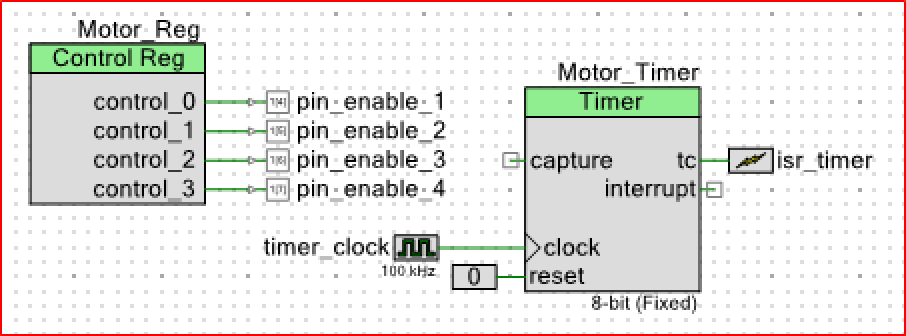
\includegraphics[width=\textwidth]{Softwaredesign/CoinSensor/graphics/TopDesign-MotorControl.png}
    \caption{PSoC top design MotorControl}
    \label{fig:MotorControl_PSoC_Design}
    \end{figure}
    Dette er motor driver som styrer CoinDispenserens aksepter og avvis funksjonalitet, så vel som balldispenseren. Den er laget ved hjelp av et kontrollregister som er koblet til stepper motorens spoler, det brukes en timer til å kontrollere motorens hastighet for å forhindre "busy waiting". Driveren består av en state machine som inneholder de forskjellige trinnene, når staten endres skrives det nye verdier til registret som fører til at steppermotoren tar et skritt.
    
    \begin{figure}
        \centering
        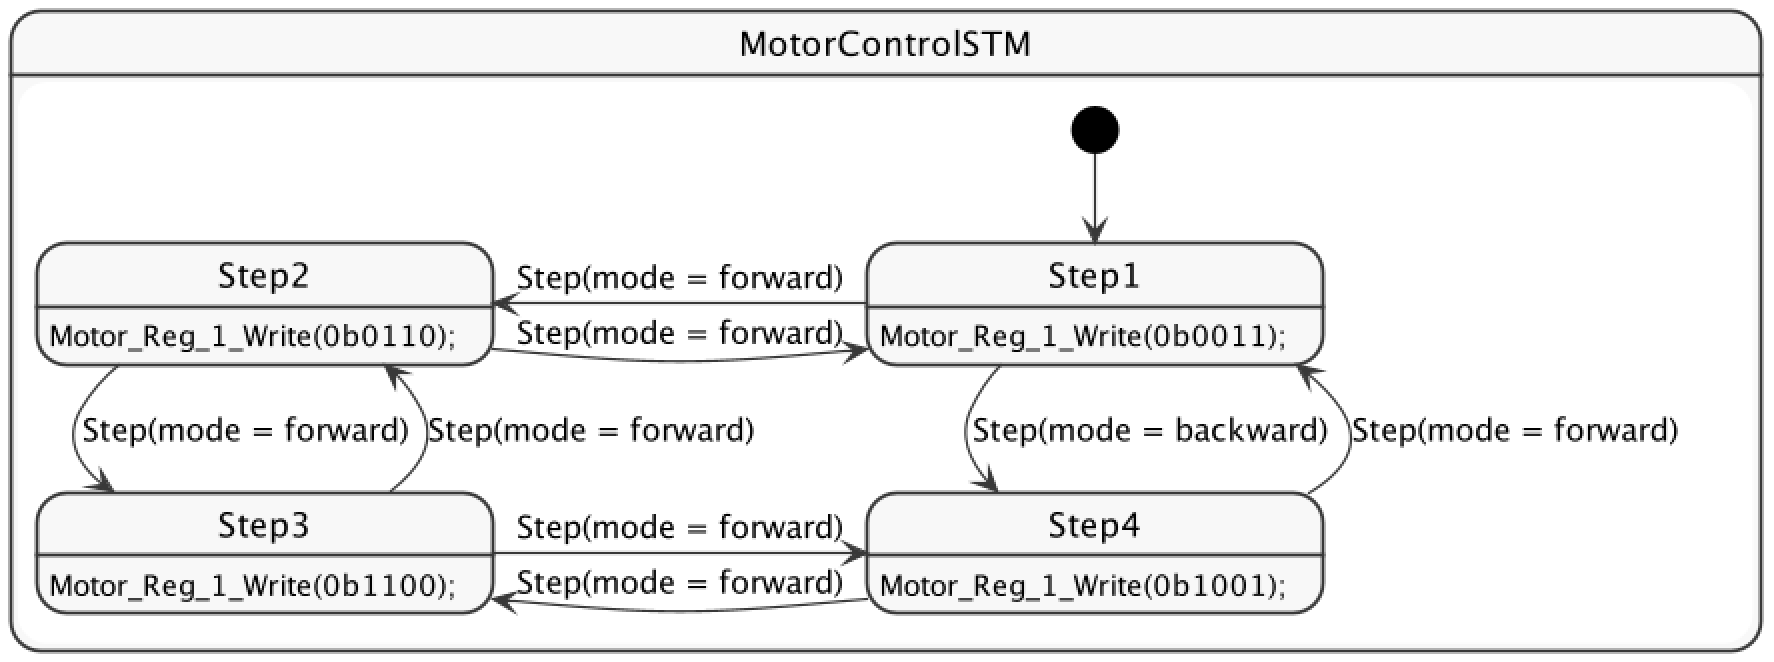
\includegraphics[width=\textwidth]{Softwaredesign/CoinSensor/graphics/MotorControlSTM.png}
        \caption{Statemachine for the motor controller}
        \label{fig:MotorControlSTM}
    \end{figure}
    
    \subsubsection{Implementering}
Dette modulet består av flere funksjoner men det er valgt å kun inkludere en motor kontroll funksjon siden alle virker på samme måte.


{\textbf{step}}\\
\begin{lstlisting}[caption={Stepper motor kontroller},style=customc,label={lst:dispenserControlFunction}]
void step(int mode)
{

    switch (nextStep)
    {
        case 0 :
        {
            Motor_Reg_1_Write(0b0011);
            if(mode == -1)
            {
                nextStep = 3;
            }
            else
            {
                nextStep += mode;
            }
        }
            break;
        case 1 :
        {
            Motor_Reg_1_Write(0b0110);
            nextStep += mode;
        }
            break;
        case 2 :
        {
            Motor_Reg_1_Write(0b1100);
            nextStep += mode;
        }
            break;
        case 3 :
        {
            Motor_Reg_1_Write(0b1001);
            if(mode == 1)
            {
                nextStep = 0;
            }
            else
            {
                nextStep += mode;
            }
        }
            break;
    }
}
\end{lstlisting}
Dette er den viktigste funksjonen i motor controll, den har 4 states som den stepper gjennom hver gang step funksjonen blir kalt. nextStep blir oppdatert etter hvilket mode den blir kaldt i. Det vil si den stepper fra 1 til 4 hvis den der i forward mode og fra 4 til 1 hvis den er i reverse.

{\textbf{Interrupt}}\\
\begin{lstlisting}[caption={Example of a motorcontrol function},style=customc,label={lst:dispenserControlFunction}]
CY_ISR(Motor_Timer_I_handler)
{
    readyForNextStep = true;
}
\end{lstlisting}
Dette er funksjonen som kalles når PSoC mottar et interrupt fra motorstyringstimeren. Det forhindrer at motoren sitter fast i motorstyringsfunksjonene. Dette betyr også at motor hastigheten styres av timer hastigheten.


\begin{lstlisting}[caption={Example of a motorcontrol function},style=customc,label={lst:dispenserControlFunction}]
void Rotate90()
{
    int x = 0;
    while(x < 512)
    {
        while(!readyForNextStep)
        {
        };
        step(Forward);
        readyForNextStep = false;
        x++;
    }
};
\end{lstlisting}
Dette er et eksempel på en motorstyringsfunksjon, de er alle konstruert på samme måte. De venter i while loopen til timer interruptet setter readyForNextStep til true og fortsetter rundt for loopen til motoren har flyttet riktig mengde grader
\end{document}